\begin{figure}[H]
  \begin{center}
  	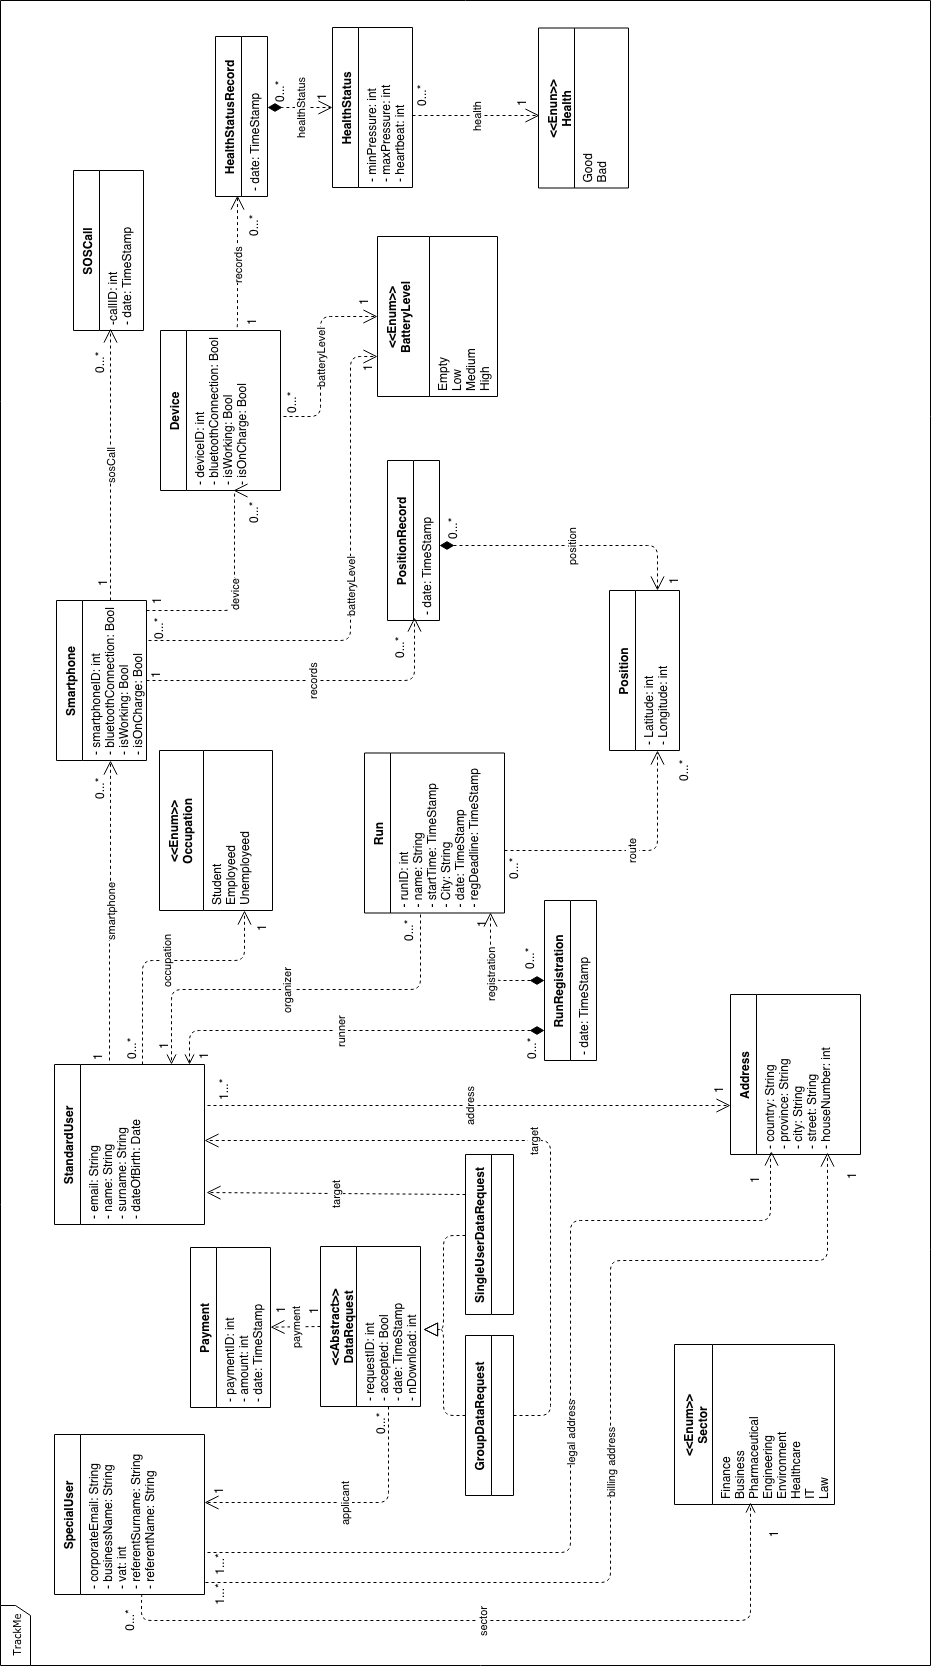
\includegraphics[height=0.45\paperheight]{./img/Class_Diagram.png}
		\caption{\textit{Class diagram} of the structure of the system-to-be.}
    \hspace{0.05\linewidth}
    \centering
		\label{classDiagram}
    \end{center}
\end{figure}

\newpage

% Settings for Alloy code listing.
\lstset{
    language=alloy,
    numbers=left,
    numberstyle=\tiny,
    stepnumber=2,
    tabsize=4,
    keywordstyle=\color{alloy-keyword}\bfseries,
    commentstyle=\color{alloy-comment},
    stringstyle=\color{alloy-string},
    basicstyle=\small\fontfamily{pcr}\selectfont, % Courier font family
}

% Includes the Alloy model file.
\lstinputlisting{./files/Alloy.als}
%\vfill
